\chapter{Comprehension of plural and clitic /s/}\label{chapter08}

As explained in detail in Section \ref{section02_2}, two comprehension studies are part of this book. This chapter presents the second of these studies on the comprehension of subphonemic differences in word-final /s/. The two studies differ in two main regards. First, the comprehension study described in Chapter \ref{chapter07} made use of real words in isolation, the comprehension study presented in this chapter uses pseudowords embedded within sentences as stimuli. Second, the first comprehension study used non-morphemic and plural word-final /s/, while this second study uses plural, \textit{is}-, and \textit{has}-clitic word-final /s/. As in the previous comprehension study, effects on comprehension were tested using a number-decision task in a mouse-tracking paradigm. Considering extant models and approaches of speech perception and comprehension, \textsc{H comp}, the ``Mismatch Hypothesis", again is explored. However, taking into account the findings of the first comprehension study, reaction times are not investigated in the present study. That is, only the second part of the hypothesis is considered: If listeners make use of subphonemic durational differences in the comprehension of different types of word-final /s/, then a mismatch of subphonemic detail and intended meaning is expected to lead to deviated mouse trajectories.

\section{Methdology}\label{section08_1}

\subsection{Participants}\label{section08_1_1}

42 native speakers of New Zealand English took part in the experiment. Their mean age was 22.5 years, ranging from 18 to 54. Eight participants identified as multilingual. The experiment took place at the University of Canterbury, Christ-church, New Zealand, from December 2020 to March 2021.

\subsection{Materials}\label{section08_1_2}

The speech materials consisted of pseudowords embedded within sentences. The pseudowords used are those forty-eight described in Section \ref{section03_1_2}. I repeat all pseudowords in Table \ref{tab:8.1} for convenience.

\begin{table}\fontsize{10}{11}
\caption{Orthographic (\textit{orth.}) and phonological (\textit{phon.}) representations of all pseudowords used in the number-decision task}
\label{tab:8.1}
\centering
\begin{tabular}{lcccccc} 
\lsptoprule
~              & /glɪ/          & /prʌ/          & /pli:/          & /clu:/          & /blaʊ/          & /gleɪ/           \\ 
\midrule
\textit{orth.} & \textit{glips} & \textit{prups} & \textit{pleeps} & \textit{cloops} & \textit{bloups} & \textit{glaips}  \\
\textit{phon.} & /glɪps/        & /prʌps/        & /pli:ps/        & /klu:ps/        & /blaʊps/        & /gleɪps/         \\ 
\midrule
\textit{orth.} & \textit{glits} & \textit{pruts} & \textit{pleets} & \textit{cloots} & \textit{blouts} & \textit{glaits}  \\
\textit{phon.} & /glɪts/        & /prʌts/        & /pli:ts/        & /klu:ts/        & /blaʊts/        & /gleɪts/         \\ 
\midrule
\textit{orth.} & \textit{gliks} & \textit{pruks} & \textit{pleeks} & \textit{clooks} & \textit{blouks} & \textit{glaiks}  \\
\textit{phon.} & /glɪks/        & /prʌks/        & /pli:ks/        & /klu:ks/        & /blaʊks/        & /gleɪks/         \\ 
\midrule
\textit{orth.} & \textit{glifs} & \textit{prufs} & \textit{pleefs} & \textit{cloofs} & \textit{bloufs} & \textit{glaifs}  \\
\textit{phon.} & /glɪfs/        & /prʌfs/        & /pli:fs/        & /klu:fs/        & /blaʊfs/        & /gleɪfs/         \\
\lspbottomrule
\end{tabular}
\end{table}

All pseudowords were embedded into short context sentences of either simple past, simple progressive, or simple perfect tense. Additionally, the remaining context disambiguated between plural and non-plural contexts. In sentences with simple past tense, the agents were two aliens of the same kind (see \ref{ex:8.1a:sentence8.1a} \& \ref{ex:8.1b:sentence8.1b}) doing something together or to each other. This ensured a plural reading of the context. In sentences with simple progressive tense, agents were a single alien doing something to or with another alien in object position (see \ref{ex:8.2a:sentence8.2a} \& \ref{ex:8.2b:sentence8.2b}). In sentences with simple perfect tense, agents were single aliens who had done something to or with another alien in object position (see \ref{ex:8.3a:sentence8.3a} \& \ref{ex:8.3b:sentence8.3b}). That is, for the \textit{is}- and \textit{has}-clitic, the following verb ensured the pertinent clitic reading of the context. Almost exclusively irregular verbs were used to create the context sentences to ensure no ambiguities between them. Twenty-four contexts per type of /s/ were created, resulting in a total number of seventy-two context sentences. See the \ref{Supplementary Material} for a list of all verbs and contexts.

\ex.
\label{ex:8.1a:sentence8.1a}
	The \textit{glips} ate their lunch together.
	
\ex.
\label{ex:8.1b:sentence8.1b}
	The \textit{glips} blew a kiss to each other.

\ex.
\label{ex:8.2a:sentence8.2a}
	The \textit{glip’s} eating cake with the bloup. 

\ex.
\label{ex:8.2b:sentence8.2b}
	The \textit{glip’s} blowing a kiss to the bloup.
	
\ex.
\label{ex:8.3a:sentence8.3a}
    The \textit{glip’s} eaten the bloup’s lunch.
	
\ex.
\label{ex:8.3b:sentence8.3b}
	The \textit{glip’s} blown kisses to the blout every day of their marriage.

The context sentences were made into a reading list, which was then read and recorded three times by a trained native speaker of New Zealand English. Recordings took place at the soundproof booth of the Department of Linguistics at the University of Tübingen. The recordings were sampled at 44.1 kHz, 16 bit.

For each sentence the best of the three recordings was chosen by manual inspection. First, all recordings were analysed using Praat following the segmentation conventions laid out in Section \ref{section04_1_4}. Recordings with production errors, e.g. laughter, stutter or vocal fry, or segmentation difficulties, e.g. the absence of a stop release, were dismissed. Second, the speaking rate of sentences was measured using a Praat script (\cite{deJong2008}) and then analysed in R. As the contexts used in the current experiment differ in length, i.e. in number of syllables, speaking rate appeared to be a more appropriate measurement of similarity across utterances as compared to duration itself as used in the previous two experiments. Speaking rate was computed as number of syllables divided by utterance duration. The resulting mean speaking rate was $3.024$ with a standard deviation of $0.551$. Lastly, for each sentence, the iteration closest to the mean speaking rate was chosen for further use in the experiment resulting in a final mean speaking rate of $3.021$ with a standard deviation of $0.380$.

Then, the final /s/ duration of all items was manipulated in such a way that it corresponded to the mean /s/ duration for plural, \textit{is}-, and \textit{has}-clitic /s/ found in the reference study by \citet{Plag2017}. That is, in the case of a plural context such as \ref{ex:8.1a:sentence8.1a} the duration of the final /s/ was changed to 283 ms, while in the case of \textit{is}-clitic contexts such as \ref{ex:8.2a:sentence8.2a} the duration of the final /s/ was changed to 261 ms, and in the case of \textit{has}-clitic contexts such as \ref{ex:8.3a:sentence8.3a} the duration of the final /s/ was changed to 253 ms. These versions are manipulated so that their /s/ durations match those of previous findings. Thus, these items are referred to as ``matched" items.

For ``mismatched" items, /s/ durations were changed as follows. For each plural context, two new versions were created. One contained the typical duration of an \textit{is}-clitic /s/, while the other one contained the typical duration of a \textit{has}-clitic /s/. For each \textit{is}-clitic and \textit{has}-clitic context, a new version was created with the duration of a typical plural /s/. The final number of contexts and their /s/ durations are given in Table \ref{tab:8.2}.

\begin{table}\fontsize{9}{10}
\caption{Number of versions per type of word-final /s/ and their /s/ durations. Mean values are taken from \citet{Plag2017}}
\label{tab:8.2}
\centering
\begin{tabular}{llll}
\lsptoprule
\textbf{~}                  & \begin{tabular}[c]{@{}l@{}}Version 1: \\matched\end{tabular}                   & \begin{tabular}[c]{@{}l@{}}Version 2: \\mismatched\end{tabular}               & \begin{tabular}[c]{@{}l@{}}Version 3: \\mismatched\end{tabular}                 \\
\midrule
\textit{is}-clitic context  & \begin{tabular}[c]{@{}l@{}}mean of \textit{is}-clitic /s/ \\261~ms\end{tabular}  & \begin{tabular}[c]{@{}l@{}}mean of plural /s/ \\283~ms\end{tabular}             & ~                                                                               \\
\midrule
\textit{has}-clitic context & \begin{tabular}[c]{@{}l@{}}mean of \textit{has}-clitic /s/ \\253~ms\end{tabular} & \begin{tabular}[c]{@{}l@{}}mean of plural /s/ \\283~ms\end{tabular}             & ~                                                                               \\
\midrule
plural context              & \begin{tabular}[c]{@{}l@{}}mean of plural /s/ \\283~ms\end{tabular}              & \begin{tabular}[c]{@{}l@{}}mean of \textit{is}-clitic /s/ \\261~ms\end{tabular} & \begin{tabular}[c]{@{}l@{}}mean of \textit{has}-clitic /s/ \\253~ms\end{tabular} \\
\lspbottomrule
\end{tabular}
\end{table}

\subsection{Procedure}\label{section08_1_3}

Similar to the experiment in Chapter \ref{chapter07}, the number-decision task was conducted in OpenSesame using the mousetrap plugin for mouse-tracking (\cite{Kieslich2017}). First, participants were introduced to the task at hand. They were told that in the following experiment they had to decide whether a sentence is about the action of two identical aliens, i.e. aliens of the same species and name, or about the action of one alien. They were told to mouse-click on the matching ``one" or ``two or more" button, respectively, in the top left and top right corner of the screen. Figure \ref{fig:8_1} illustrates what participants saw on screen for each trial. The participants were told that if they do not decide on either option within a certain amount of time, the next trial started automatically. Each participant started with five practice trials.

\begin{figure}
    \centering
    \includegraphics[width=0.7\textwidth]{figures/fig8.1.png}
    \caption{Option display during the comprehension experiment. The mouse cursor indicates the position the mouse was reset to in each trial}
    \label{fig:8_1}
\end{figure}

Each trial was preceded by a stretch of silence of 450 ms accompanied by a white screen. Then, one of the recordings was played, with reaction time and mouse-tracking measurement starting at the onset of the recording. Participants were given a window of 4500 ms starting after the onset of the recording to react, after that a time-out was recorded. The next trial then started automatically 5000 ms after the onset of the previous recording, starting with the next inter-trial white screen. Mouse-tracks were recorded with a frequency of 100 Hz.

\section{Analysis}\label{section08_2}

The analysis of the present data is similar to the analysis of the mouse-tracking data in the comprehension study on non-morphemic and plural word-final /s/ in Chapter \ref{chapter07}. First, mouse-tracking data was extracted, spatially transformed, and time-normalised with n = 140 time steps using the mousetrap package (\cite{Kieslich2019}) in R. Figure \ref{fig:8_2} shows the aggregated mean trajectory of the spatially transformed and time-normalised mouse-tracks in the lower left panel. The panel on top gives the overall distribution of all X coordinates, with a peak visible around a value of $0$. The panel on the right displays the overall distribution of all Y coordinates, with a peak around a value of $380$. As in Chapter \ref{chapter07}, the positions of the peaks corresponds to the position at which the mouse cursor started for each trial.

\begin{figure}
    \centering
    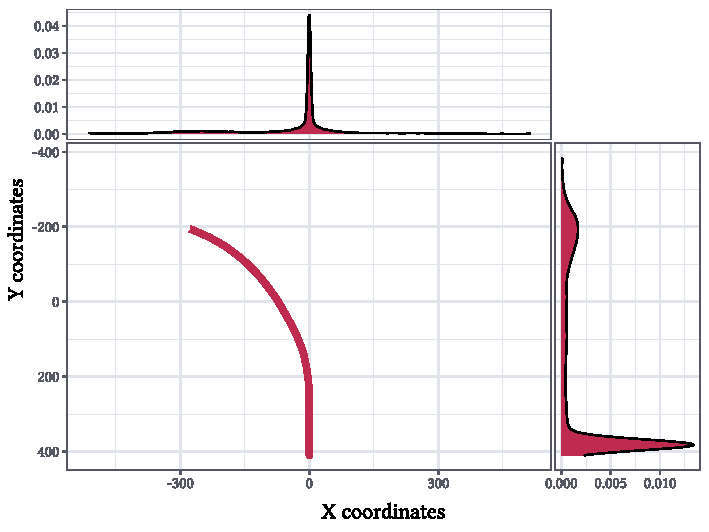
\includegraphics[]{figures/fig8.2.pdf}
    \caption{Mean trajectory of all spatially adjusted and time-normalised mouse-tracks (lower left), and density distribution of X and Y coordinates (on top and on the right, respectively)}
    \label{fig:8_2}
\end{figure}

Then, X and Y coordinates were extracted using the \texttt{mtqgam} package (\cite{Schmitz2021mtqgam}). As in Section \ref{section07_2_3}, the sign of the coordinate data was reversed to allow for a straightforward interpretation. An example of the resulting data structure is given in Table \ref{tab:8.3}.

\begin{table}\fontsize{9}{10}
\caption{Example of the data format for a matched trial}
\label{tab:8.3}
\centering
\begin{tabular}{rrrrrr} 
\lsptoprule
\textsc{order} & \textsc{trialNumber} & \textsc{time}      & \textsc{x\_coordinate} & \textsc{y\_coordinate} & \textsc{condition}  \\ 
\midrule
1     & 1           & 0         & 0             & -380.000      & matched    \\
…     & …           & …         & …             & …             & …          \\
9     & 1           & 201.9568  & 2.000         & -380.000      & matched    \\
10    & 1           & 227.2014  & 3.440         & -379.560      & matched    \\
11    & 1           & 252.4460  & 6.734         & -375.266      & matched    \\
…     & …           & …         & …             & …             & …          \\
110   & 1           & 2751.6619 & 72.487        & 90.160        & matched    \\
111   & 1           & 2776.9065 & 139.647       & 120.597       & matched    \\
…     & …           & …         & …             & …             & …          \\
130   & 1           & 3256.5540 & 274.000       & 199.000       & matched    \\
131   & 1           & 3281.7986 & 274.000       & 199.000       & matched    \\
\lspbottomrule
\end{tabular}
\end{table}

Finally, the prepared data set was analysed using additive quantile regression models (QGAMs; \cite{Fasiolo2021}). 

\subsection{Fitted models}\label{section08_2_1}

The complete set of coordinate data (n = 1,017,800) was split into four separate data sets. Recall that there were three types of word-final /s/ involved in this study, i.e. plural, \textit{is}-, and \textit{has}-clitic /s/. Targets in plural context sentences were once manipulated to bear the mismatched /s/ duration of an \textit{is}-clitic, and once to bear the mismatched /s/ duration of a \textit{has}-clitic. An overview of the four subsets and the contexts they contain is given in Table \ref{tab:8.4}.

\begin{table}\fontsize{10}{11}
\caption{Overview of the four subsets used in the QGAM modelling process. Each subset contains mouse-track coordinate data of durationally matched and mismatched stimuli. Within each subset, the type of context is kept constant, while the manipulation of the pertinent word-final /s/ either corresponds to a match or mismatch in duration. Subset names contain information on the type of context (first subscript letter) and the /s/ duration that constitutes a mismatch (second subscript letter)}
\label{tab:8.4}
\centering
\begin{tabular}{llll} 
\lsptoprule
Subset name               & Condition  & Context             & /s/ duration           \\ 
\midrule
\multirow{2}{*}{\textsc{subset\textsubscript{IP}}} & matched    & \textit{is}-clitic  & \textit{is}-clitic   \\
                          & mismatched & \textit{is}-clitic  & plural               \\ 
\midrule
\multirow{2}{*}{\textsc{subset\textsubscript{HP}}} & matched    & \textit{has}-clitic & \textit{has}-clitic  \\
                          & mismatched & \textit{has}-clitic & plural               \\ 
\midrule
\multirow{2}{*}{\textsc{subset\textsubscript{PI}}} & matched    & plural              & plural               \\
                          & mismatched & plural              & \textit{is}-clitic   \\ 
\midrule
\multirow{2}{*}{\textsc{subset\textsubscript{PH}}} & matched    & plural              & plural               \\
                          & mismatched & plural              & \textit{has}-clitic  \\
\lspbottomrule
\end{tabular}
\end{table}

\textsc{subset\textsubscript{IP}} thus contained results on \textit{is}-clitic contexts with either \textit{is}-clitic /s/ or plural /s/ durations (n = 260,400). \textsc{subset\textsubscript{HP}} contained results on \textit{has}-clitic contexts with either \textit{has}-clitic /s/ or plural /s/ durations (n = 229,600). \textsc{subset\textsubscript{PI}} contained results on plural contexts with either plural /s/ or \textit{is}-clitic /s/ durations (n = 263,900). \textsc{subset\textsubscript{PH}}, finally, contained results on plural contexts with either plural /s/ or \textit{has}-clitic /s/ durations (n = 263,900). Similar to the analysis of mouse-tracks in the comprehension study on non-morphemic and plural /s/ presented in Section \ref{section07_2_3}, the individual subsets were created in order to determine whether a mismatch of context and word-final /s/ influenced mouse-tracks to a significant extent. While this is also possible with the specification of interaction terms in the QGAM formula, it was again decided against this method due to the high computational costs as well as due to the increased complexity of model interpretation. 

Two sets of QGAMs were fitted to each of the four subsets. One set of QGAMs was fitted to X coordinates, one set of QGAMs was fitted to Y coordinates. I aimed at estimating the conditional quantiles corresponding to $\tau=0.1,0.3,0.5,0.7$ and $0.9$. Thus, each set of QGAMs consisted of five individual QGAMs, one for each of the five quantiles. In total, ten QGAMs for each of the four subsets were fitted, that is five for X coordinates and five for Y coordinates. This resulted in a total number of forty QGAMs.

Taking into account the low number of incorrectly answered trials in the data of Chapter \ref{chapter07}, I checked the amount of data points for which the wrong answer was given in the present data. Again, only few trials with wrong answers, i.e. about 9 \% (n = 89,740), were found. It was decided to exclude \textsc{correct} as a variable for the QGAM model formula, and to only use data on correctly answered trials instead. This led to slightly smaller data sets, i.e. n = 243,600 for \textsc{subset\textsubscript{IP}}; n = 193,340 for \textsc{subset\textsubscript{HP}}; n = 246,820 for \textsc{subset\textsubscript{PI}}; and n = 244,300 for \textsc{subset\textsubscript{PH}}. An overview of all variables contained in the four subsets is given in Table \ref{tab:8.5}. See Section \ref{section07_2_1} for the definitions of all covariates.

\begin{table}\fontsize{10}{11}
\caption{Summary of the dependent variables and the numerical and categorical predictors in the four subsets}
\label{tab:8.5}
\centering
\begin{tabular}{lrrrr}
\lsptoprule
Subset(s) & Mean              & St. Dev.           & Min      & Max      \\
\midrule
\textsc{subset\textsubscript{IP}}  & 50.326            & 135.957            & -511.000 & 512.000  \\
\textsc{subset\textsubscript{HP}}  & 48.251            & 142.696            & -511.000 & 512.000  \\
\textsc{subset\textsubscript{PI}}  & 32.086            & 142.656            & -512.000 & 511.000  \\
\textsc{subset\textsubscript{PH}}  & 32.507            & 141.780            & -512.000 & 511.000  \\
\textsc{subset\textsubscript{IP}}  & -173.983          & 250.326            & -410.000 & 384.000  \\
\textsc{subset\textsubscript{HP}}  & -160.199          & 253.547            & -410.000 & 384.000  \\
\textsc{subset\textsubscript{PI}}  & -181.272          & 245.044            & -410.000 & 384.000  \\
\textsc{subset\textsubscript{PH}}  & -177.168          & 248.281            & -410.000 & 384.000  \\
\midrule
Subset(s) & Mean              & St. Dev.           & Min      & Max      \\
\midrule
all       & 70.500            & 40.414             & 1.000    & 140.000  \\
\midrule
Subset(s) & \multirow{1}{*}{Levels}            & ~                  & ~        & ~        \\
\midrule
all       & \multirow{1}{*}{24}                & ~                  & ~        & ~        \\
all       & \multirow{1}{*}{42}                & ~                  & ~        & ~        \\
\midrule
Subset(s) & \multirow{1}{*}{Levels}            &                    &          &          \\
\midrule
\textsc{subset\textsubscript{IP}}  & \multicolumn{2}{l}{\texttt{matched}: 121940} & \multicolumn{2}{l}{\texttt{mismatched}: 121660}    \\

\textsc{subset\textsubscript{HP}}  & \multicolumn{2}{l}{\texttt{matched}: 97020} & \multicolumn{2}{l}{\texttt{mismatched}: 96320}    \\

\textsc{subset\textsubscript{PI}}  & \multicolumn{2}{l}{\texttt{matched}: 123760} & \multicolumn{2}{l}{\texttt{mismatched}: 123060}    \\

\textsc{subset\textsubscript{PH}}  & \multicolumn{2}{l}{\texttt{matched}: 121800} & \multicolumn{2}{l}{\texttt{mismatched}: 122500}    \\
\lspbottomrule
\end{tabular}
\end{table}

All QGAMs used the same model formula. The dependent variable was either \textsc{x\_coordinate} or \textsc{y\_coordinate}. \textsc{condition} was introduced as parametric term. \textsc{order} was given as smooth term with the default \textit{k}-value of $9$, and \textsc{item} and \textsc{subject} were included as random smooth terms. Checks revealed that the \textit{k}-value of the \textsc{order} smooth term was too low. However, as in Section \ref{section07_2_2_2}, it was found that no matter the \textit{k}-value, the effect of all covariates remained unchanged. Following \citet{Wood2017}, it was therefore, again, decided to not re-fit the computationally costly QGAMs. The final data set as well as the analysis and results discussed in the following sections can be found in the \ref{Supplementary Material}. In the following, the results of the modelling process will be presented.

\subsection{Results}\label{section08_2_2}

A significant effect of \textsc{condition} was found 24 times across all forty models. The smooth term of \textsc{order} as well as the random smooth terms of \textsc{item} and \textsc{subject} reached significance in all models. The overall model fit is rather high with a mean deviance explained of $\overline{D}=58.75$ \%. Across all four data sets, QGAMs fitted to Y coordinates showed overall higher rates of deviance explained ($\overline{D}=68.29$ \%) than their X coordinate counterparts ($\overline{D}=49.21$ \%). For all four sets of QGAMs, the QGAM fitted to the $0.5$ quantile showed the lowest rate of deviance explained ($\overline{D}=44.69$ \%), while the QGAMs fitted to the more extreme quantiles showed the highest rates of deviance explained ($\overline{D}=75.41$ \% and $\overline{D}=72.06$ \%).

\subsubsection{\textsc{subset\textsubscript{IP}}}\label{section08_2_2_1}

The effects found in the QGAMs fitted to the X and Y coordinates of \textsc{subset\textsubscript{IP}} are given in Table \ref{tab:8.6}. The model estimates of these and all subsequent QGAMs are given in the \ref{Supplementary Material}. Note that here and in the following, I will refrain from discussing the effects of the smooth terms as they are not the main interest of investigation. 

There are significant effects of \textsc{condition} in two QGAMs fitted to X coordinate data and in two QGAMs fitted to Y coordinate data. For both types of coordinates, these effects are found for $\tau=0.7$ and $\tau=0.9$. The effects are illustrated by Figure \ref{fig:8_3} Where a significant effect is found for X coordinates, tracks of mismatched trials are further to the left as compared to tracks of matched trials. For Y coordinates, the effect of condition leads to coordinates further up for mismatched trials. Recall that due to the use of conditional quantiles in QGAMs, the estimates shown in Figure \ref{fig:8_3} and similar plots illustrate the nature of an effect taking into account a certain quantity of the overall data. Such plots do not illustrate the positions of mouse-tracks at certain points of their trajectory.

\begin{table}\fontsize{9}{10}
\caption{Summary of the effects found in the QGAMs fitted to the X and Y coordinates of \textsc{subset\textsubscript{IP}}. Significance codes: `***' $p < 0.001$, `**' $p < 0.01$, `*' $p < 0.05$}
\label{tab:8.6}
\centering
\begin{tabular}{lrrrrrrrrrrr}
\lsptoprule
~                   & \multicolumn{5}{c}{X coordinates} & \multicolumn{1}{c}{}    & \multicolumn{5}{c}{Y coordinates}                               \\
\midrule
\multicolumn{1}{r}{quantiles:}          & 0.1        & 0.3        & 0.5        & 0.7        & 0.9 & ~        & 0.1        & 0.3        & 0.5        & 0.7        & 0.9         \\
\midrule
Parametric Terms    & \textbf{~} & \textbf{~} & \textbf{~} & \textbf{~} & \textbf{~} & \textbf{~} & \textbf{~} & \textbf{~} & \textbf{~} & \textbf{~}  \\
\midrule
(Intercept)         & ***        & ***        & ***        & ***        & *** & ~        & ***        & ***        & ***        & ***        & n.s.          \\
\textsc{condition}\texttt{mismatched} & n.s.       & n.s.          & n.s.        & ***        & *** & ~        & n.s.       & n.s.        & n.s.        & **        & ***         \\
\midrule
Smooth Terms        & \textbf{~} & \textbf{~} & \textbf{~} & \textbf{~} & \textbf{~} & \textbf{~} & \textbf{~} & \textbf{~} & \textbf{~} & \textbf{~}  \\
\midrule
\textsc{order}               & ***        & ***        & ***        & ***        & *** & ~        & ***        & ***        & ***        & ***        & ***         \\
\midrule
Random Smooth Terms & \textbf{~} & \textbf{~} & \textbf{~} & \textbf{~} & \textbf{~} & \textbf{~} & \textbf{~} & \textbf{~} & \textbf{~} & \textbf{~}  \\
\midrule
\textsc{item}                & ***        & ***        & ***        & ***        & *** & ~        & ***        & ***        & ***        & ***        & ***         \\
\textsc{subject}             & ***        & ***        & ***        & ***        & *** & ~        & ***        & ***        & ***        & ***        & ***        \\
\lspbottomrule
\end{tabular}
\end{table}

\begin{figure}
    \centering
    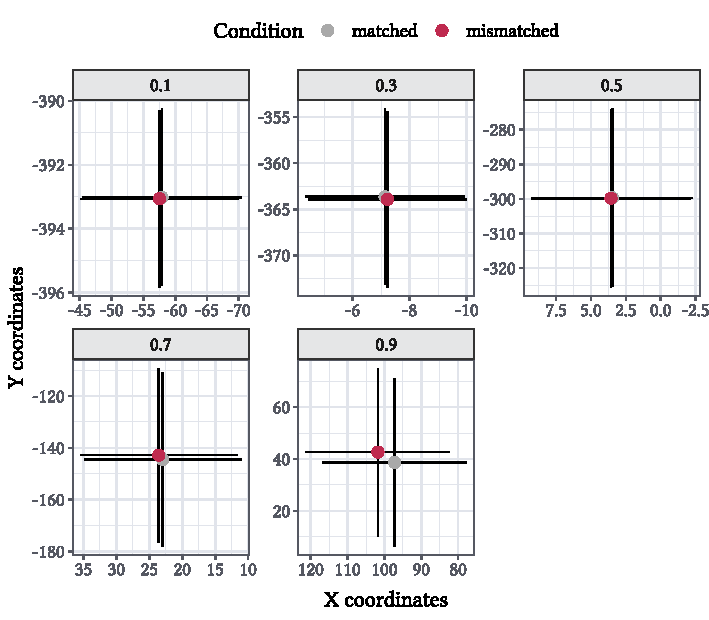
\includegraphics[]{figures/fig8.3.pdf}
    \caption{Effect of \textsc{condition} as found in the QGAMs modelled to the X and Y coordinates of \textsc{subset\textsubscript{IP}}. The lines indicate the confidence intervals of the estimated X and Y coordinate values}
    \label{fig:8_3}
\end{figure}

\subsubsection{\textsc{subset\textsubscript{HP}}}\label{section08_2_2_2}

For \textsc{subset\textsubscript{HP}}, the found effects are given in Table \ref{tab:8.7}. The effect of \textsc{condition} reaches significance in three QGAMs fitted to X coordinates, i.e. in the $\tau=0.1,0.7$ and $0.9$ quantiles. For Y coordinates, significant effects are found in all QGAMs but the QGAM fitted to the $\tau=0.9$ quantile. The effects are illustrated in Figure \ref{fig:8.4}. For X coordinates in $\tau=0.1$, the effect of \textsc{condition} leads to coordinates further to the right. Taking into account more data, the effect is reversed in $\tau=0.7$ and $0.9$, i.e. coordinates of mismatched trials are further left. The effect of \textsc{condition} on Y values is similar across all quantiles. That is, mismatched trials show further up Y coordinates.

\begin{table}\fontsize{9}{10}
\caption{Summary of the effects found in the QGAMs fitted to the X and Y coordinates of \textsc{subset\textsubscript{HP}}. Significance codes: `***' $p < 0.001$, `**' $p < 0.01$, `*' $p < 0.05$}
\label{tab:8.7}
\centering
\begin{tabular}{lrrrrrrrrrrr}
\lsptoprule
~                   & \multicolumn{5}{c}{X coordinates}       & \multicolumn{1}{c}{}                       & \multicolumn{5}{c}{Y coordinates}                               \\
\midrule
\multicolumn{1}{r}{quantiles:}          & 0.1        & 0.3        & 0.5        & 0.7        & 0.9 & ~       & 0.1        & 0.3        & 0.5        & 0.7        & 0.9         \\
\midrule
Parametric Terms    & \textbf{~} & \textbf{~} & \textbf{~} & \textbf{~} & \textbf{~} & \textbf{~} & \textbf{~} & \textbf{~} & \textbf{~} & \textbf{~}  \\
\midrule
(Intercept)         & ***        & ***        & ***        & ***        & *** & ~       & ***        & ***        & ***        & ***        & **          \\
\textsc{condition}\texttt{mismatched} & ***       & n.s.          & n.s.        & **        & ***  & ~      & *       & ***        & ***        & ***        & n.s.         \\
\midrule
Smooth Terms        & \textbf{~} & \textbf{~} & \textbf{~} & \textbf{~} & \textbf{~} & \textbf{~} & \textbf{~} & \textbf{~} & \textbf{~} & \textbf{~}  \\
\midrule
\textsc{order}               & ***        & ***        & ***        & ***        & ***   & ~     & ***        & ***        & ***        & ***        & ***         \\
\midrule
Random Smooth Terms & \textbf{~} & \textbf{~} & \textbf{~} & \textbf{~} & \textbf{~} & \textbf{~} & \textbf{~} & \textbf{~} & \textbf{~} & \textbf{~}  \\
\midrule
\textsc{item}                & ***        & ***        & ***        & ***        & ***  & ~      & ***        & ***        & ***        & ***        & ***         \\
\textsc{subject}             & ***        & ***        & ***        & ***        & ***  & ~      & ***        & ***        & ***        & ***        & ***        \\
\lspbottomrule
\end{tabular}
\end{table}

\begin{figure}
    \centering
    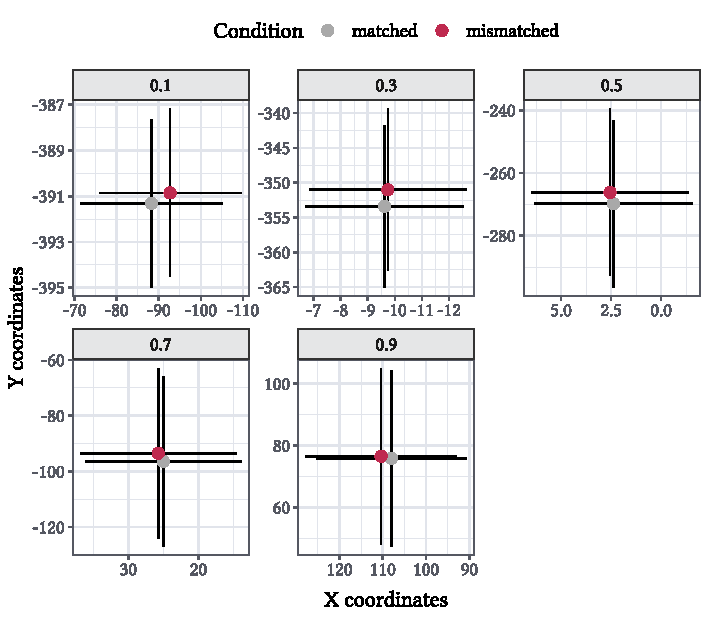
\includegraphics[]{figures/fig8.4.pdf}
    \caption{Effect of \textsc{condition} as found in the QGAMs modelled to the X and Y coordinates of \textsc{subset\textsubscript{HP}}. The lines indicate the confidence intervals of the estimated X and Y coordinate values}
    \label{fig:8_4}
\end{figure}

\subsubsection{\textsc{subset\textsubscript{PI}}}\label{section08_2_2_3}

Table \ref{tab:8.8} presents the effects found for QGAMs fitted to the \textsc{subset\textsubscript{PI}} data. A significant effect of \textsc{condition} is found in quantiles $\tau=0.1,0.3$ and $0.5$ for X coordinates, and in all quantiles but $\tau=0.1$ for Y coordinates. The effects are displayed in Figure \ref{fig:8_5}. Where the effect of \textsc{condition} is significant for X values, coordinates of mismatched trials are further right. For Y coordinates, the effect of \textsc{condition} comes with coordinates further down for mismatched trial coordinates.

\begin{table}\fontsize{9}{10}
\caption{Summary of the effects found in the QGAMs fitted to the X and Y coordinates of \textsc{subset\textsubscript{PI}}. Significance codes: `***' $p < 0.001$, `**' $p < 0.01$, `*' $p < 0.05$}
\label{tab:8.8}
\centering
\begin{tabular}{lrrrrrrrrrrr}
\lsptoprule
~                   & \multicolumn{5}{c}{X coordinates}    & \multicolumn{1}{c}{}                          & \multicolumn{5}{c}{Y coordinates}                               \\
\midrule
\multicolumn{1}{r}{quantiles:}          & 0.1        & 0.3        & 0.5        & 0.7        & 0.9  & ~      & 0.1        & 0.3        & 0.5        & 0.7        & 0.9         \\
\midrule
Parametric Terms    & \textbf{~} & \textbf{~} & \textbf{~} & \textbf{~} & \textbf{~} & \textbf{~} & \textbf{~} & \textbf{~} & \textbf{~} & \textbf{~}  \\
\midrule
(Intercept)         & ***        & n.s.         & ***        & ***        & ***    & ~    & ***        & ***        & ***        & ***        & n.s.          \\
\textsc{condition}\texttt{mismatched} & n.s.       & n.s.          & n.s.        & ***        & *** & ~       & ***       & ***        & ***        & ***        & n.s.         \\
\midrule
Smooth Terms        & \textbf{~} & \textbf{~} & \textbf{~} & \textbf{~} & \textbf{~} & \textbf{~} & \textbf{~} & \textbf{~} & \textbf{~} & \textbf{~}  \\
\midrule
\textsc{order}               & ***        & ***        & ***        & ***        & ***  & ~      & ***        & ***        & ***        & ***        & ***         \\
\midrule
Random Smooth Terms & \textbf{~} & \textbf{~} & \textbf{~} & \textbf{~} & \textbf{~} & \textbf{~} & \textbf{~} & \textbf{~} & \textbf{~} & \textbf{~}  \\
\midrule
\textsc{item}                & ***        & ***        & ***        & ***        & ***  & ~      & ***        & ***        & ***        & ***        & ***         \\
\textsc{subject}             & ***        & ***        & ***        & ***        & ***  & ~      & ***        & ***        & ***        & ***        & ***        \\
\lspbottomrule
\end{tabular}
\end{table}

\begin{figure}
    \centering
    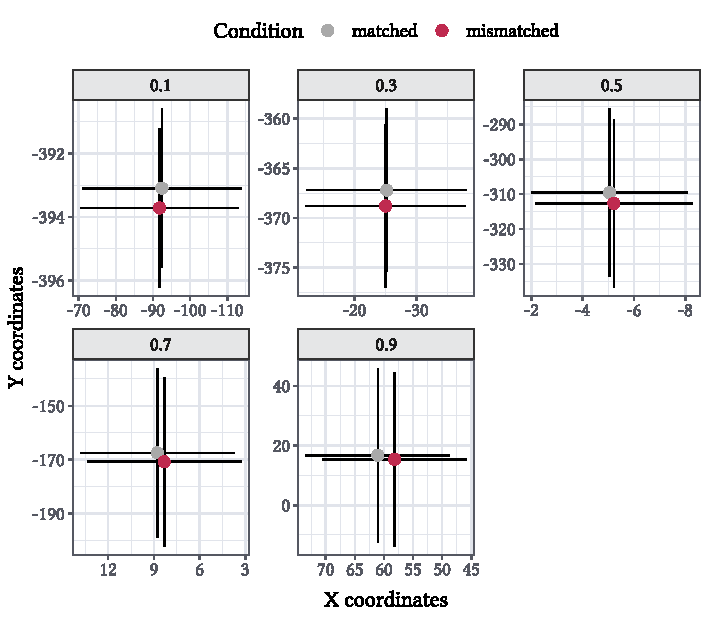
\includegraphics[]{figures/fig8.5.pdf}
    \caption{Effect of \textsc{condition} as found in the QGAMs modelled to the X and Y coordinates of \textsc{subset\textsubscript{PI}}. The lines indicate the confidence intervals of the estimated X and Y coordinate values}
    \label{fig:8_5}
\end{figure}

\subsubsection{\textsc{subset\textsubscript{PH}}}\label{section08_2_2_4}

Finally, the effects found in the QGAMs fitted to the X and Y coordinates of the \textsc{subset\textsubscript{PH}} data are given in Table \ref{tab:8.9} \textsc{condition} shows a significant effect on X coordinates in quantiles $\tau=0.5,0.7$ and $0.9$. For Y coordinates, a significant effect is found in all quantiles but $\tau=0.9$. The effects are illustrated in Figure \ref{fig:8_5}. For X coordinates, the effect of \textsc{condition} comes with coordinates further left for mismatched trials. For Y coordinates, the effect of \textsc{condition} leads to coordinates lower down for mismatched trials.

\begin{table}\fontsize{9}{10}
\caption{Summary of the effects found in the QGAMs fitted to the X and Y coordinates of \textsc{subset\textsubscript{PH}}. Significance codes: `***' $p < 0.001$, `**' $p < 0.01$, `*' $p < 0.05$}
\label{tab:8.9}
\centering
\begin{tabular}{lrrrrrrrrrrr}
\lsptoprule
~                   & \multicolumn{5}{c}{X coordinates}       & \multicolumn{1}{c}{}                       & \multicolumn{5}{c}{Y coordinates}                               \\
\midrule
\multicolumn{1}{r}{quantiles:}          & 0.1        & 0.3        & 0.5        & 0.7        & 0.9  & ~       & 0.1        & 0.3        & 0.5        & 0.7        & 0.9         \\
\midrule
Parametric Terms    & \textbf{~} & \textbf{~} & \textbf{~} & \textbf{~} & \textbf{~} & \textbf{~} & \textbf{~} & \textbf{~} & \textbf{~} & \textbf{~}  \\
\midrule
(Intercept)         & ***        & n.s.         & ***        & ***        & *** & ~       & ***        & ***        & ***        & ***        & n.s.          \\
\textsc{condition}\texttt{mismatched} & **       & ***          & ***        & n.s.        & n.s.    & ~    & n.s.       & *        & ***        & ***        & ***         \\
\midrule
Smooth Terms        & \textbf{~} & \textbf{~} & \textbf{~} & \textbf{~} & \textbf{~} & \textbf{~} & \textbf{~} & \textbf{~} & \textbf{~} & \textbf{~}  \\
\midrule
\textsc{order}               & ***        & ***        & ***        & ***        & ***   & ~     & ***        & ***        & ***        & ***        & ***         \\
\midrule
Random Smooth Terms & \textbf{~} & \textbf{~} & \textbf{~} & \textbf{~} & \textbf{~} & \textbf{~} & \textbf{~} & \textbf{~} & \textbf{~} & \textbf{~}  \\
\midrule
\textsc{item}                & ***        & ***        & ***        & ***        & ***   & ~     & ***        & ***        & ***        & ***        & ***         \\
\textsc{subject}             & ***        & ***        & ***        & ***        & ***  & ~      & ***        & ***        & ***        & ***        & ***        \\
\lspbottomrule
\end{tabular}
\end{table}

\begin{figure}
    \centering
    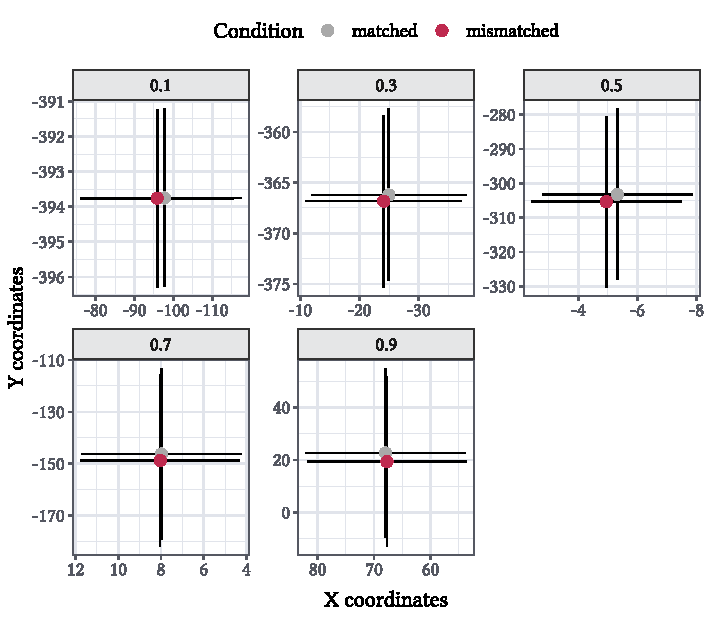
\includegraphics[]{figures/fig8.6.pdf}
    \caption{Effect of \textsc{condition} as found in the QGAMs modelled to the X and Y coordinates of \textsc{subset\textsubscript{PH}}. The lines indicate the confidence intervals of the estimated X and Y coordinate values}
    \label{fig:8_6}
\end{figure}

\subsubsection{Overall results}\label{section08_2_2_5}

An overview of significant deviations found for the coordinates of mismatched stimuli trials across all quantiles and subsets is given in Table \ref{tab:8.10}. Considering the overall influence of \textsc{condition}, one can make two general observations. First, Y coordinates of mismatched stimuli trials are higher and, with the exception of $\tau=0.1$ for \textsc{subset\textsubscript{HP}}, further to the left if a mismatch is caused by a plural /s/ duration, as is the case in \textsc{subset\textsubscript{IP}} and \textsc{subset\textsubscript{HP}}. Second, Y coordinates of mismatched stimuli trials are lower if a mismatch is caused by an \textit{is}- or \textit{has}-clitic /s/ duration, as is the case in \textsc{subset\textsubscript{PI}} and \textsc{subset\textsubscript{PH}}, while for X coordinates no clear pattern is visible.

\begin{table}\fontsize{10}{11}
\caption{Overview of the direction of significant deviations found for coordinates in mismatched stimuli trials across all quantiles and subsets. Where no direction is given, no significant effect of \textsc{condition} was found}
\label{tab:8.10}
\centering
\begin{tabular}{ccccccccc}
\lsptoprule
\multirow{2}{*}{~} & 
\multicolumn{2}{c}{\textsc{subset\textsubscript{IP}}} & 
\multicolumn{2}{c}{\textsc{subset\textsubscript{HP}}} & 
\multicolumn{2}{c}{\textsc{subset\textsubscript{PI}}} & 
\multicolumn{2}{c}{\textsc{subset\textsubscript{PH}}}  \\
\midrule
                                   $\tau$    & X    & Y                     & X     & Y                    & X     & Y                    & X    & Y                      \\
                                       \midrule
0.1                                    & ~    & ~                     & right & higher               & ~     & lower                & left & ~                      \\
0.3                                    & ~    & ~                     & ~     & higher               & ~     & lower                & left & lower                  \\
0.5                                    & ~    & ~                     & ~     & higher               & ~     & lower                & left & lower                  \\
0.7                                    & left & higher                & left  & higher               & right & lower                & ~    & lower                  \\
0.9                                    & left & higher                & left  & ~                    & right & ~                    & ~    & lower     \\
\lspbottomrule
\end{tabular}
\end{table}

\section{Discussion}\label{section08_3}

The number-decision task presented in this chapter investigated whether listeners make use of subphonemic durational differences in comprehension. It is different to the comprehension study presented in Chapter \ref{chapter07} by several aspects. First, pseudowords instead of real words were used as items. Thus, the effects found in the present study cannot be confounded by effects of lexical storage, frequency, or relatedness which are commonly associated with real words and their representations in the mental lexicon (see Section \ref{section03_1_1}). Second, items were presented in carrier sentences and not in isolation. This was necessary to disambiguate between different types of /s/ in the long run, as the number-decision process for pseudowords cannot rely on lexical knowledge. Third, plural, \textit{is}-, and \textit{has}-clitic word-final /s/ were part of the items, while the previous comprehension study investigated non-morphemic and plural word-final /s/. By investigating different types of /s/ across studies, one obtains a more detailed picture of potential effects. Despite these differences, both comprehension studies shared the same hypothesis. Building on extant models of speech perception and comprehension, \textsc{H comp}, the ``Mismatch Hypothesis", was explored: If subphonemic durational differences are made use of, then a mismatch of subphonemic detail and intended meaning leads to a) slowed down comprehension processes, and b) deviated mouse trajectories. Part a) of the hypothesis was not investigated in the present study, as null results were found in the comprehension study of Chapter \ref{chapter07}. Thus, one question remained: Did a mismatch of subphonemic durational information lead to deviated mouse trajectories?

This question was investigated using QGAMs fitted to the X and Y coordinate data of the mouse-tracks recorded in the number-decision task. QGAMs were fitted separately for four subsets of data: 1) \textsc{subset\textsubscript{IP}}, 2) \textsc{subset\textsubscript{HP}}, 3) \textsc{subset\textsubscript{PI}}, and 4) \textsc{subset\textsubscript{PH}}, where the first subscript letter indicates the context and the second subscript letter indicates the mismatched type of /s/ (I = \textit{is}-clitic; H = \textit{has}-clitic; P = plural). In each of the subsets, trials of items with matched and mismatched /s/ duration were compared, while the items’ bases as well as the sentence the items were embedded within were kept constant. The overall results of the QGAMs show an effect of matched versus mismatched durational information across all four subsets. Taking a closer look at the nature of the found effects, one finds effects going into different directions between subsets (see Table \ref{tab:8.10}). For X coordinates, coordinate values of mismatched stimuli trials are further to the left for \textsc{subset\textsubscript{IP}}, \textsc{subset\textsubscript{HP}}, and \textsc{subset\textsubscript{PH}}. For \textsc{subset\textsubscript{PI}}, however, X coordinate values of mismatched trials are further to the right. For Y coordinates, one finds a difference between both clitic contexts and both plural contexts: Y coordinates are higher up when a mismatch is caused by a plural /s/ duration, but they are further down when the mismatch is caused by a clitic /s/ duration. Similar effects were found for QGAMs fitted post-hoc to the data for which the onset of the word-final /s/ has been heard already (see Section \ref{section07_3} for a discussion and the \ref{Supplementary Material} for model overviews).

What do these findings mean in regard to the notion of deviated mouse-tracks due to mismatched subphonemic durational information? Recall that the mouse-tracks were mirrored where applicable, that is all tracks move towards the upper left corner of the coordinate system. Thus, an ideal non-deviated trajectory would be a straight line between the mouse cursor starting position and one of the answer options. As this non-deviated straight line moves linearly towards the upper left corner, X coordinates which are further to the left or right and Y coordinates which are further up or down can be understood as deviation from that direct path. If mismatched subphonemic durational information was to cause deviation from that ideal path, one would expect X coordinates to be further to the right and Y coordinates to be lower down, as such a deviation would express the expected effect of a mismatch: As context and /s/ duration do not match up, comprehension is influenced, and the mouse-track is deviated towards the incorrect response for the pertinent trial. Taking a trial with a clitic context as an example, a mismatch is caused by the plural /s/ duration of the target word’s word-final /s/. If comprehension is influenced by this durational mismatch, one would predict mouse movement towards the plural response due to the word-final /s/ duration. Once the entire context is processed, a correct answer is given. Moving the mouse away from the incorrect towards the correct response then results in an overall more deviated mouse-track.

How do the present findings relate to this prediction of a deviated path? For X coordinates, a deviation to the right was found for $\tau=0.9$ of \textsc{subset\textsubscript{HP}} and across \textsc{subset\textsubscript{PI}}. In all other significant cases, mismatched trials showed X coordinates further to the left instead. For Y coordinates, the expected lower coordinate values were found for \textsc{subset\textsubscript{PI}} and \textsc{subset\textsubscript{PH}}, while \textsc{subset\textsubscript{IP}} and \textsc{subset\textsubscript{HP}} showed higher Y coordinate values instead. That is, only the results for \textsc{subset\textsubscript{PI}} fully meet the expected directions of deviations. \textsc{subset\textsubscript{PH}} meets the directions for Y coordinates, but not for X coordinates. The two subsets in which a mismatch is caused by a plural /s/ duration, \textsc{subset\textsubscript{IP}} and \textsc{subset\textsubscript{HP}}, show deviations of the opposite directions instead: X coordinates are mainly further to the left and Y coordinates are higher up. Nonetheless, the ``Mismatch Hypothesis" is confirmed by the overall findings: Comparing mouse-tracks of matched and mismatched stimuli trials, one finds that they significantly deviate from each other across more than half of all QGAMs. 

However, how can one explain the opposing findings between \textsc{subset\textsubscript{IP}} and \textsc{subset\textsubscript{HP}} on the one, and \textsc{subset\textsubscript{PI}} and \textsc{subset\textsubscript{HP}} on the other hand? Noticeably, the effects found within the two clitic context subsets, as well as the effects found within the two plural context subsets are mostly similar. General differences in effect directions for Y coordinates are only found between these two groups. One potential explanation that comes to mind is the overall frequency of plural and clitic /s/ in the language. In the British National Corpus (\cite{Davies2004}), \textit{is}-clitic <’s> is attested 311,146 times and \textit{has}-clitic <’s> is attested 22,816 times. For plural <s>, the most frequent entry alone, \textit{things}, has a frequency of 40,453 which is almost double the frequency of the \textit{has}-clitic. Considering just plural /s/, one finds a frequency of about 140,000 when taking into account the top ten most frequent /s/ plural forms alone. That is, plural /s/ is overall far more frequent than clitic /s/. If a pseudoword contains the duration of a plural /s/, mouse-tracks deviate differently than predicted, i.e. further to the left and further up, as plural /s/ duration is the expected duration. The plural /s/ duration is expected as it is more frequent across the language. If a pseudoword contains the duration of a clitic /s/, mouse-tracks are deviated as predicted, i.e. further down, as this is a less expected duration due to the relatively low frequency of the clitic /s/ duration. Note that this is but an idea which requires further investigation.

Overall, the present results confirm that comprehension is significantly influenced by a mismatch of subphonemic durational information in word-final /s/. This finding is in line with the results of the mouse-track analysis presented for the comprehension study in Chapter \ref{chapter07} of this book. The nature of the found deviations, however, remains unaccounted for and requires further research.

Let us now turn to the theoretical implications of the present findings. Abstractionist theories which exclude subphonemic durational information from the perception and comprehension process cannot account for the present findings (e.g. \cite{Klatt1979, McClelland1986, Norris1994, Norris2008}). If such durational differences are not perceived, they cannot be used in comprehension. As significant differences between mouse-tracks of trials with matched versus mismatched durational information were found, such abstractionist approaches cannot explain the present results.

Exemplar and hybrid models (e.g. \cite{Goldinger1996, Hawkins2001, Pierrehumbert2002, Hanique2013Aalders}) and computational models (DIANA, \cite{tenBosch2015, tenBosch2021}; LDL, \cite{Baayen2019}) could in principle account for the present results. These approaches assume the storage of subphonemic detail. Such detail can be perceived and made use of in comprehension. However, it remains unclear how exemplar and hybrid models would account for the reverse effects found for clitic versus plural contexts. Computational models, however, might be able to shed further light on this issue. Taking LDL as a starting point, one could use the phonological and semantic measures derived from an implementation such as the one given in Chapter \ref{chapter05} as predictors to model coordinate data. Considering that one of these measures apparently reflects the distinction between non-morphemic and plural /s/ (see Section \ref{section05_4}), it might very well be the case that another measure can capture the effect of durational matches and mismatches. However, for such an implementation additional steps are required. First, audio data instead of phonological triphones has to be used as input to provide information on subphonemic durational differences. Second, one has to find a way to include clitic /s/, because clitic /s/ has not been incorporated in LDL implementations yet. 

In sum, no theoretical account can straightforwardly explain the findings of the present number-decision task. Mouse-tracks are influenced by mismatched subphonemic durational information in pseudowords. However, the nature of this influence is unaccounted for: Opposing directions of effects are found when comparing mismatched trials of clitic contexts and plural contexts. An explanation for these reversed effects should be motivation for future research. Such research might benefit from new LDL implementations and derived measures. Overall, the present study showed that subphonemic durational information is used in comprehension, and that such results are found independently of effects of lexical storage, frequency, and relatedness. 
